%!TEX root = ../../super_main.tex

\section{Participant Interaction}
When opening the mobile application, the participant is presented with an initial, as seen in \figref{fig:initial_screen}. The idea with this screen is to welcome the participant to the application. Currently, it does not supply the participant with much information, but one could imagine that this view would, in future iterations, provide the participant with usable information, such as progress in the current campaign, clarification of what concepts and principals the participants must know. This screen could possibly also contain some motivational factor, provided by customers. e.g. a ``prize'' for participation.

% Initial screen
\begin{figure}[!htbp]
\begin{subfigure}[!t]{.48\textwidth}
  \centering
  
\includegraphics[width=.8\linewidth]{mockups/homepage}
  \caption{Mockup.}
  \label{fig:mockup_initial_screen}
\end{subfigure}%
\begin{subfigure}[!t]{.52\textwidth}
  \centering
  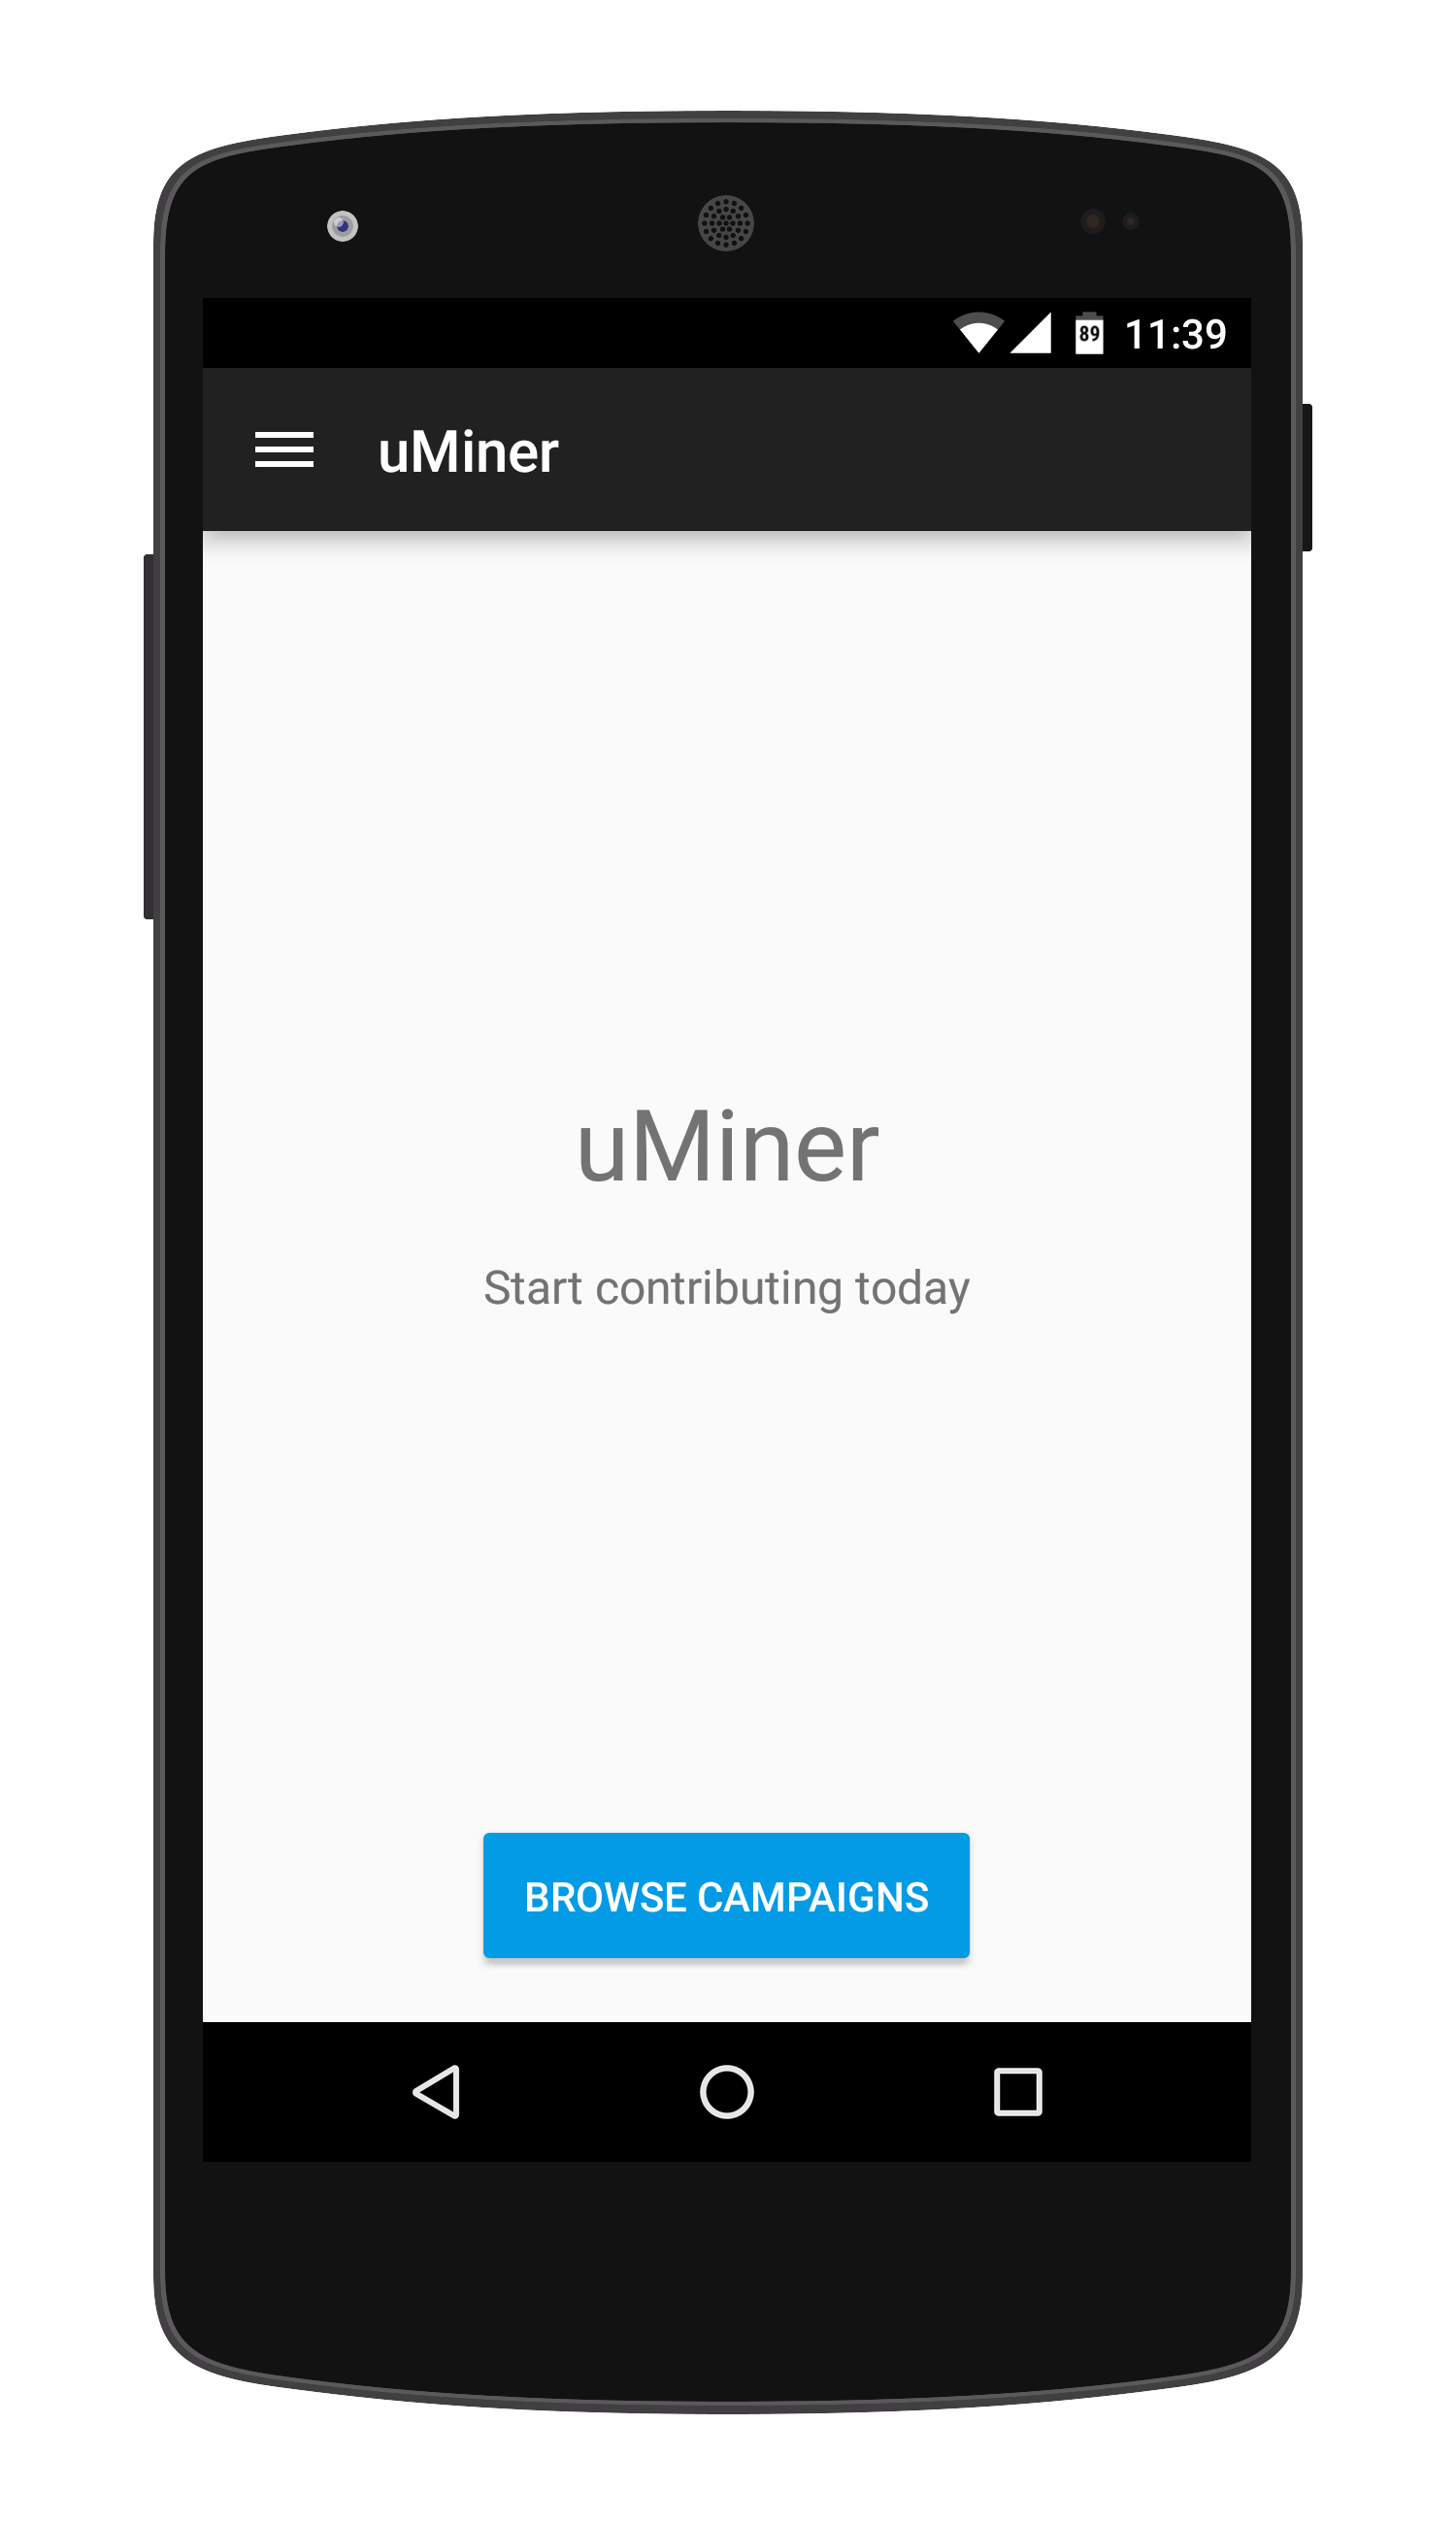
\includegraphics[width=.83\linewidth]{user_interfaces/client_uminer_home_with_phone}
  \caption{Implementation.}
  \label{fig:implementation_initial_screen}
\end{subfigure}
\caption{Initial screen of the Application.}
\label{fig:initial_screen}
\end{figure}
\FloatBarrier

To navigate to other views in the application, the participants must either use the drawer menu displayed in \figref{fig:navigation} or the \emph{browse campaigns}-button in the initial view. The navigation menu contains three elements, which will each take the participant to different parts of the application.

\begin{description}
	\item[\emph{Current campaign}] redirects the participant to a campaign specification view, as seen in \figref{fig:public_campaigns}, displaying more information about the campaign that they are currently contributing to. If the participant have not yet joined a campaign, a message will briefly be displayed on the screen, informing the participant about this.
	\item[\emph{Browse campaigns}] redirects the participant to a view containing brief information about all of the publicly available campaigns.
	\item[\emph{Join specific}] redirects the participant to a view, as seen in \figref{fig:specific_campaign}, where he/she can search for a specific campaign by providing a campaign identifier.
\end{description}

% Navigation
\begin{figure}[!htbp]
\centering
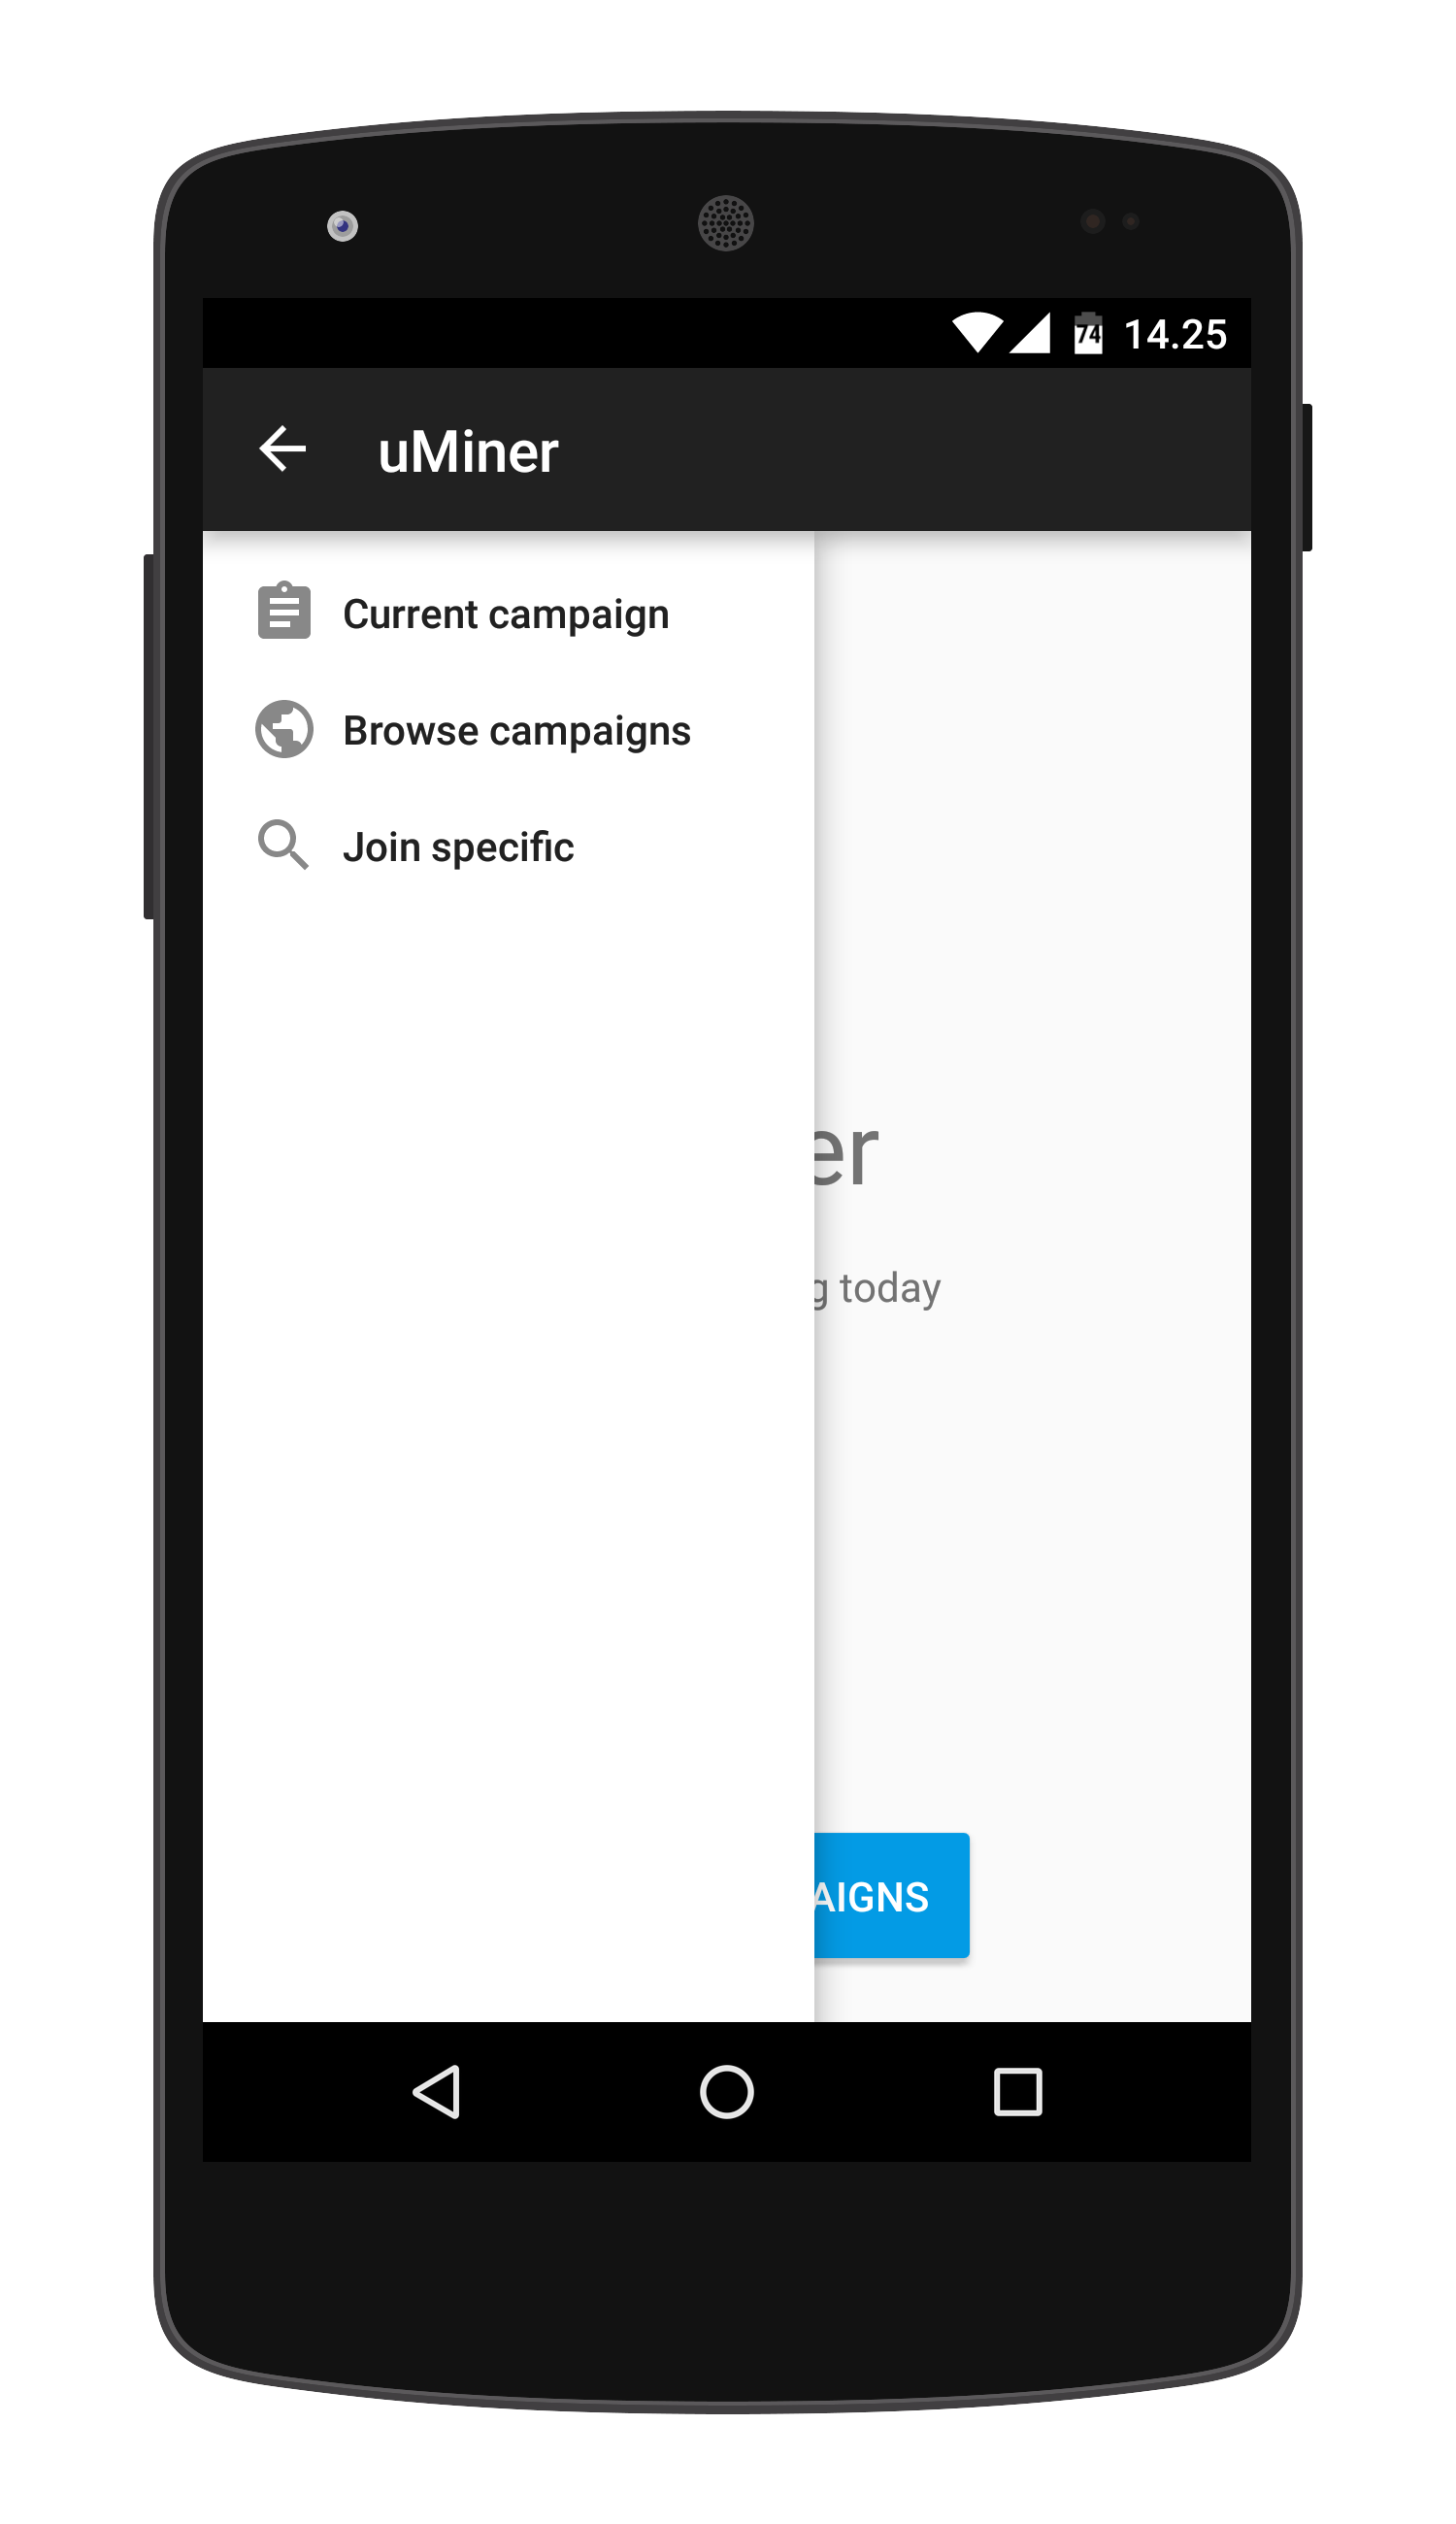
\includegraphics[width=.41\linewidth]{user_interfaces/client_drawer_menu_with_phone}
\caption{Navigation through the application.}
\label{fig:navigation}
\end{figure}
\FloatBarrier

% Publicly available campaigns
\begin{figure}[!htbp]
\begin{subfigure}[!t]{.48\textwidth}
  \centering
  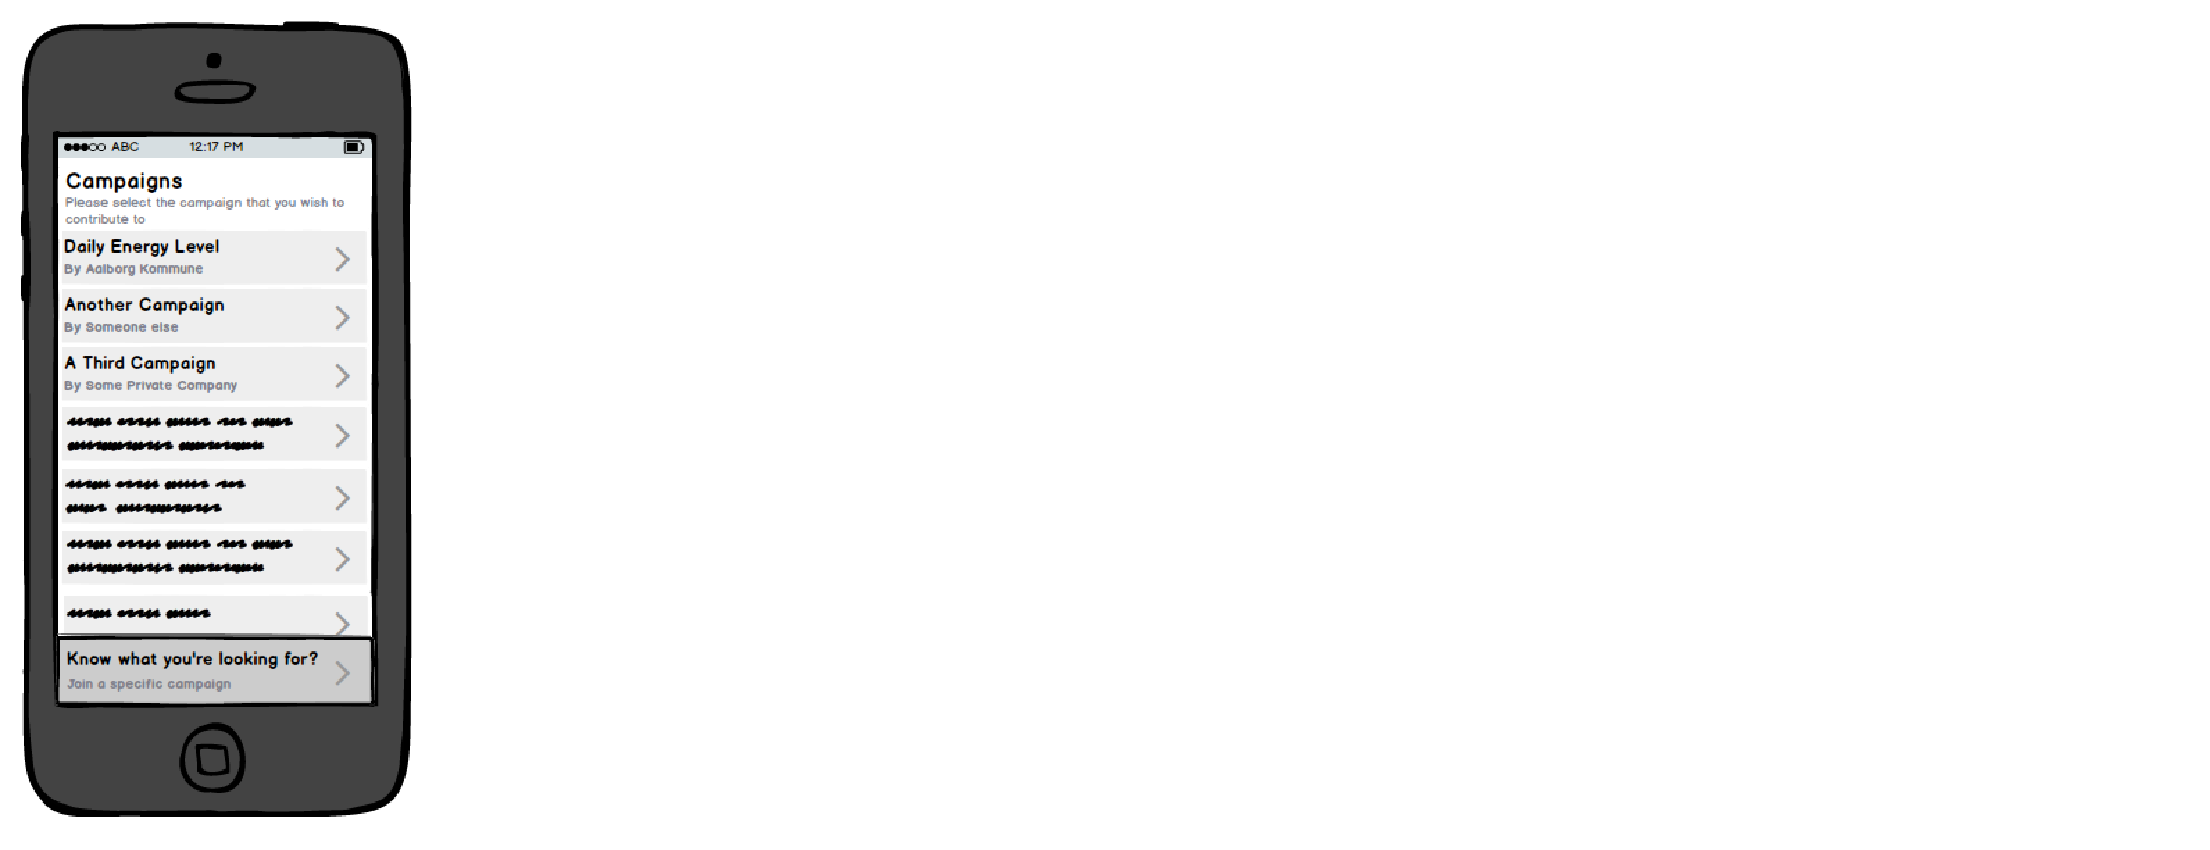
\includegraphics[width=.8\linewidth]{mockups/campaigns_list}
  \caption{Mockup.}
  \label{fig:mockup_public_campaigns}
\end{subfigure}%
\begin{subfigure}[!t]{.52\textwidth}
  \centering
  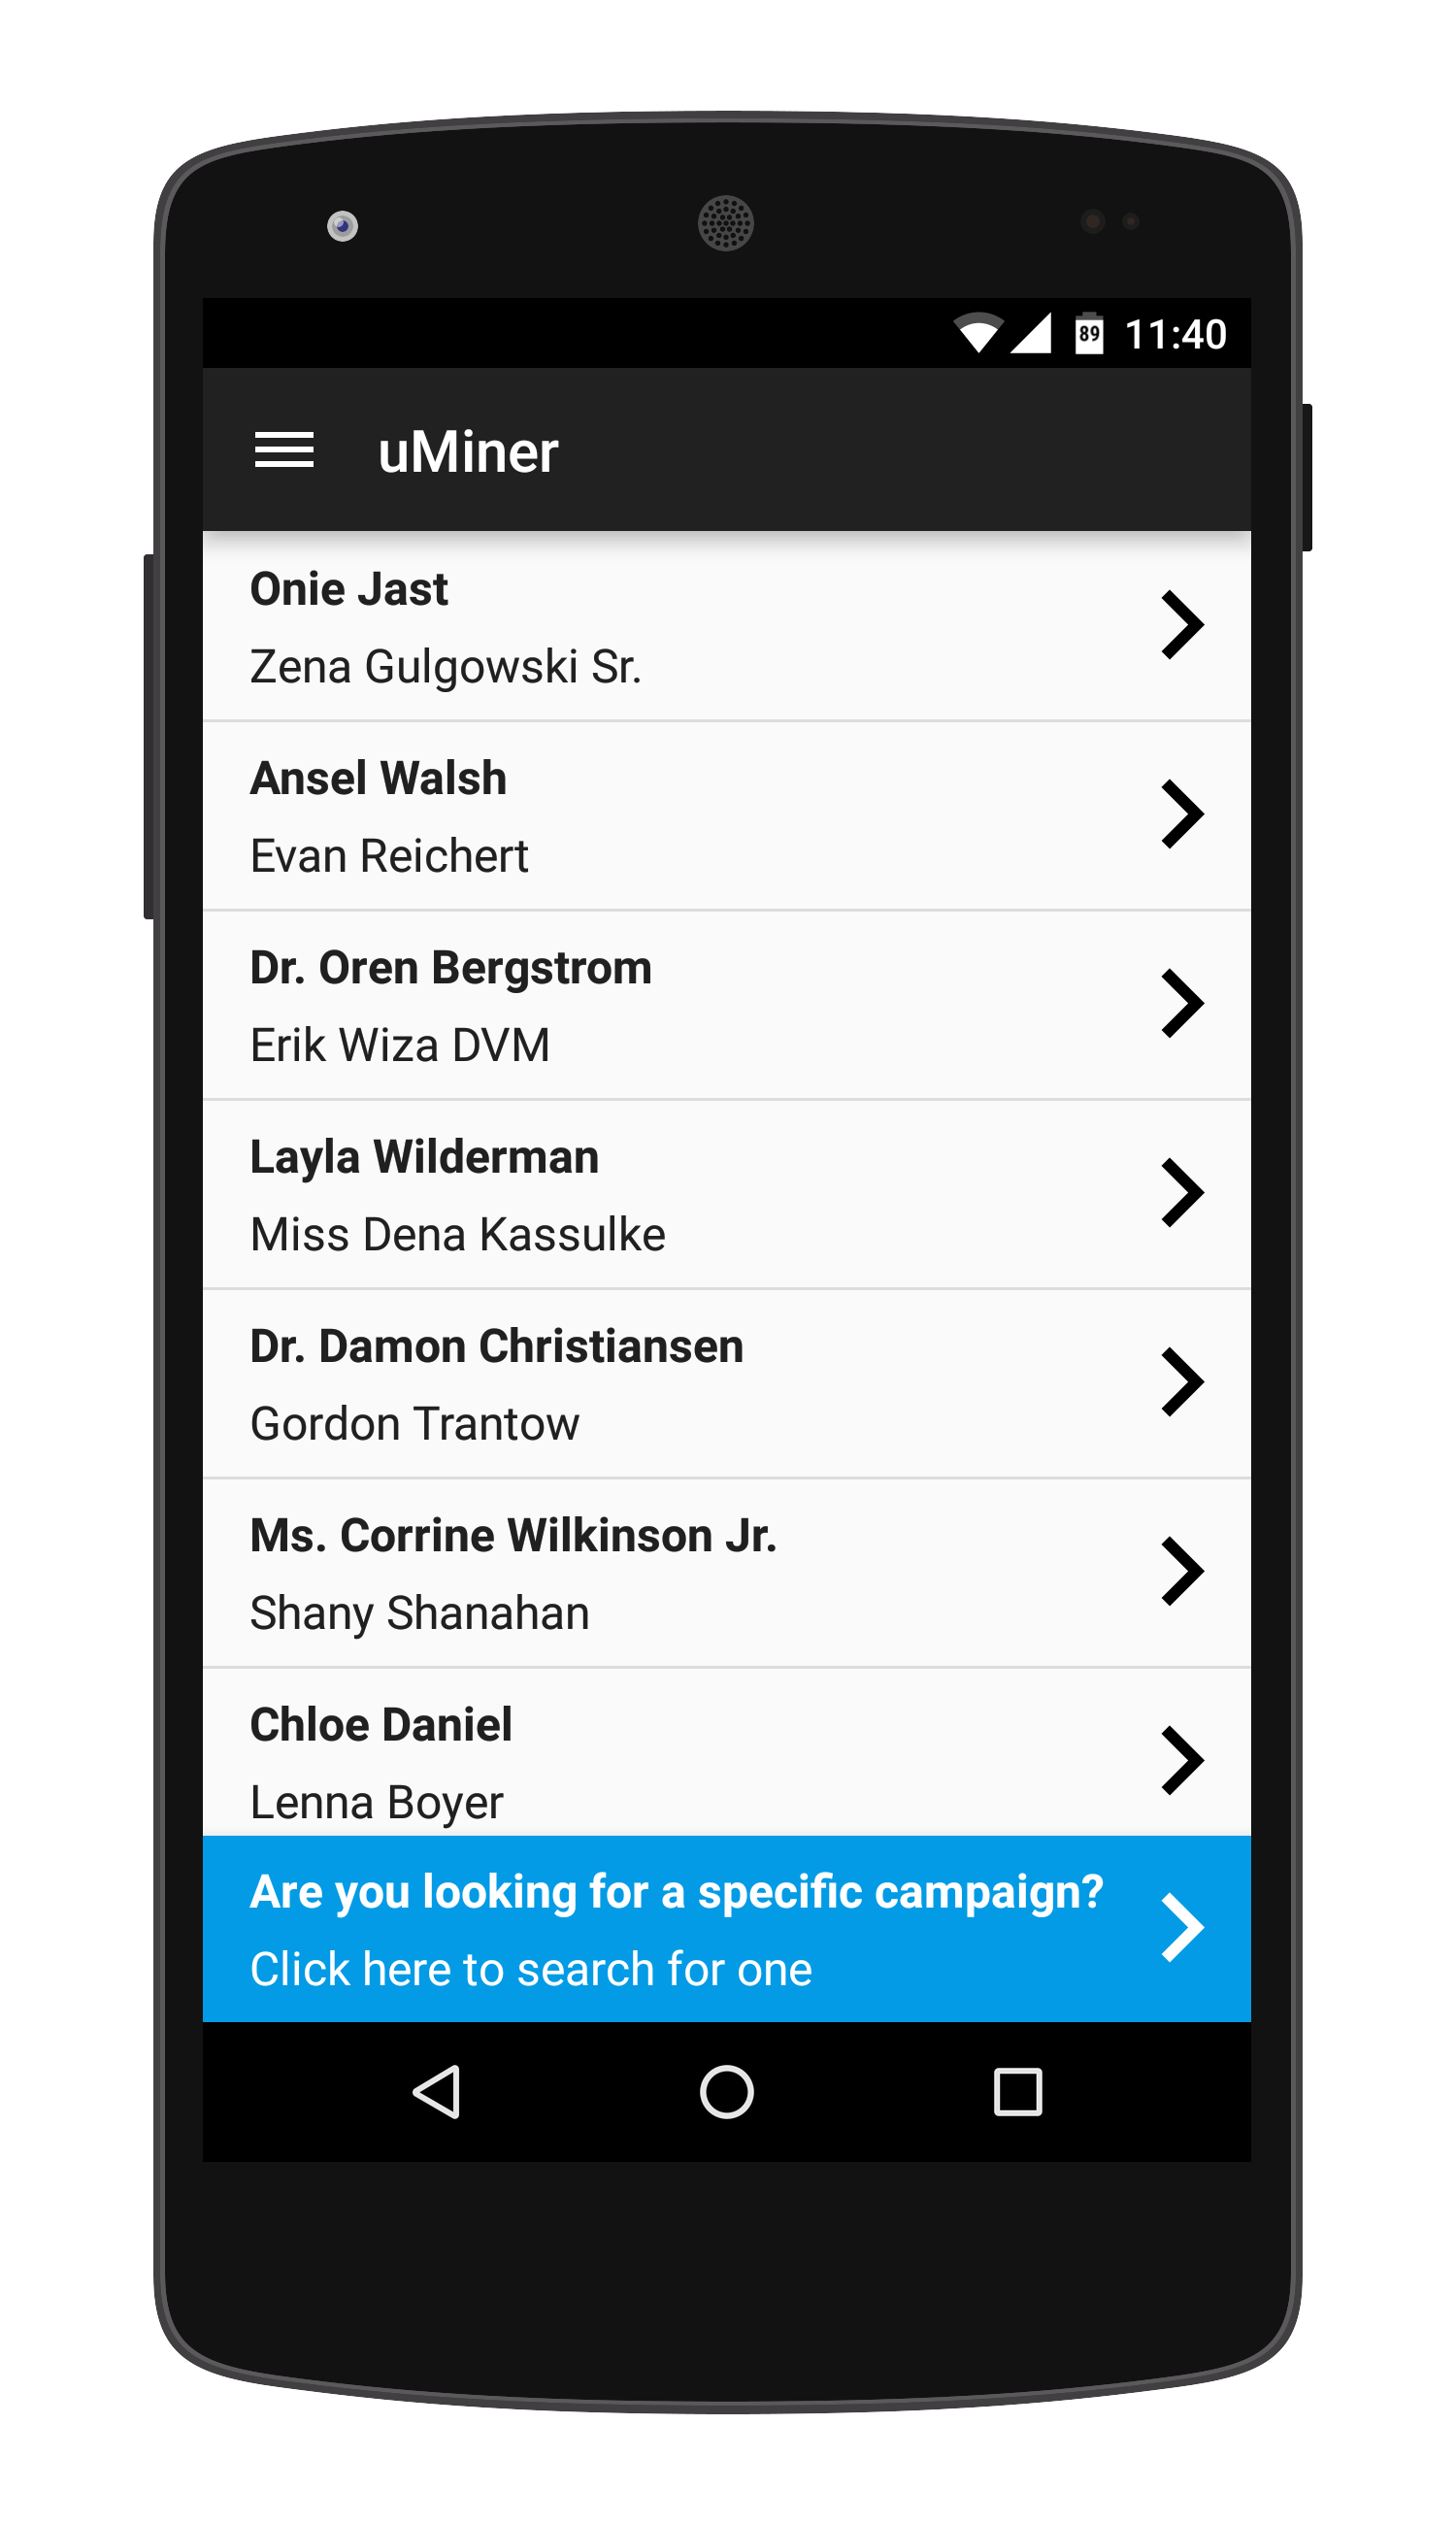
\includegraphics[width=.83\linewidth]{user_interfaces/client_public_campaigns_with_phone}
  \caption{Implementation.}
  \label{fig:implementation_public_campaigns}
\end{subfigure}
\caption{List of publicly available campaigns.}
\label{fig:public_campaigns}
\end{figure}
\FloatBarrier

% Search for a campaign through a campaign identifier
\begin{figure}[!htbp]
\begin{subfigure}[!t]{.48\textwidth}
  \centering
  
\includegraphics[width=.8\linewidth]{mockups/join_specific_campaign}
  \caption{Mockup.}
  \label{fig:mockup_specific_campaign}
\end{subfigure}%
\begin{subfigure}[!t]{.52\textwidth}
  \centering
  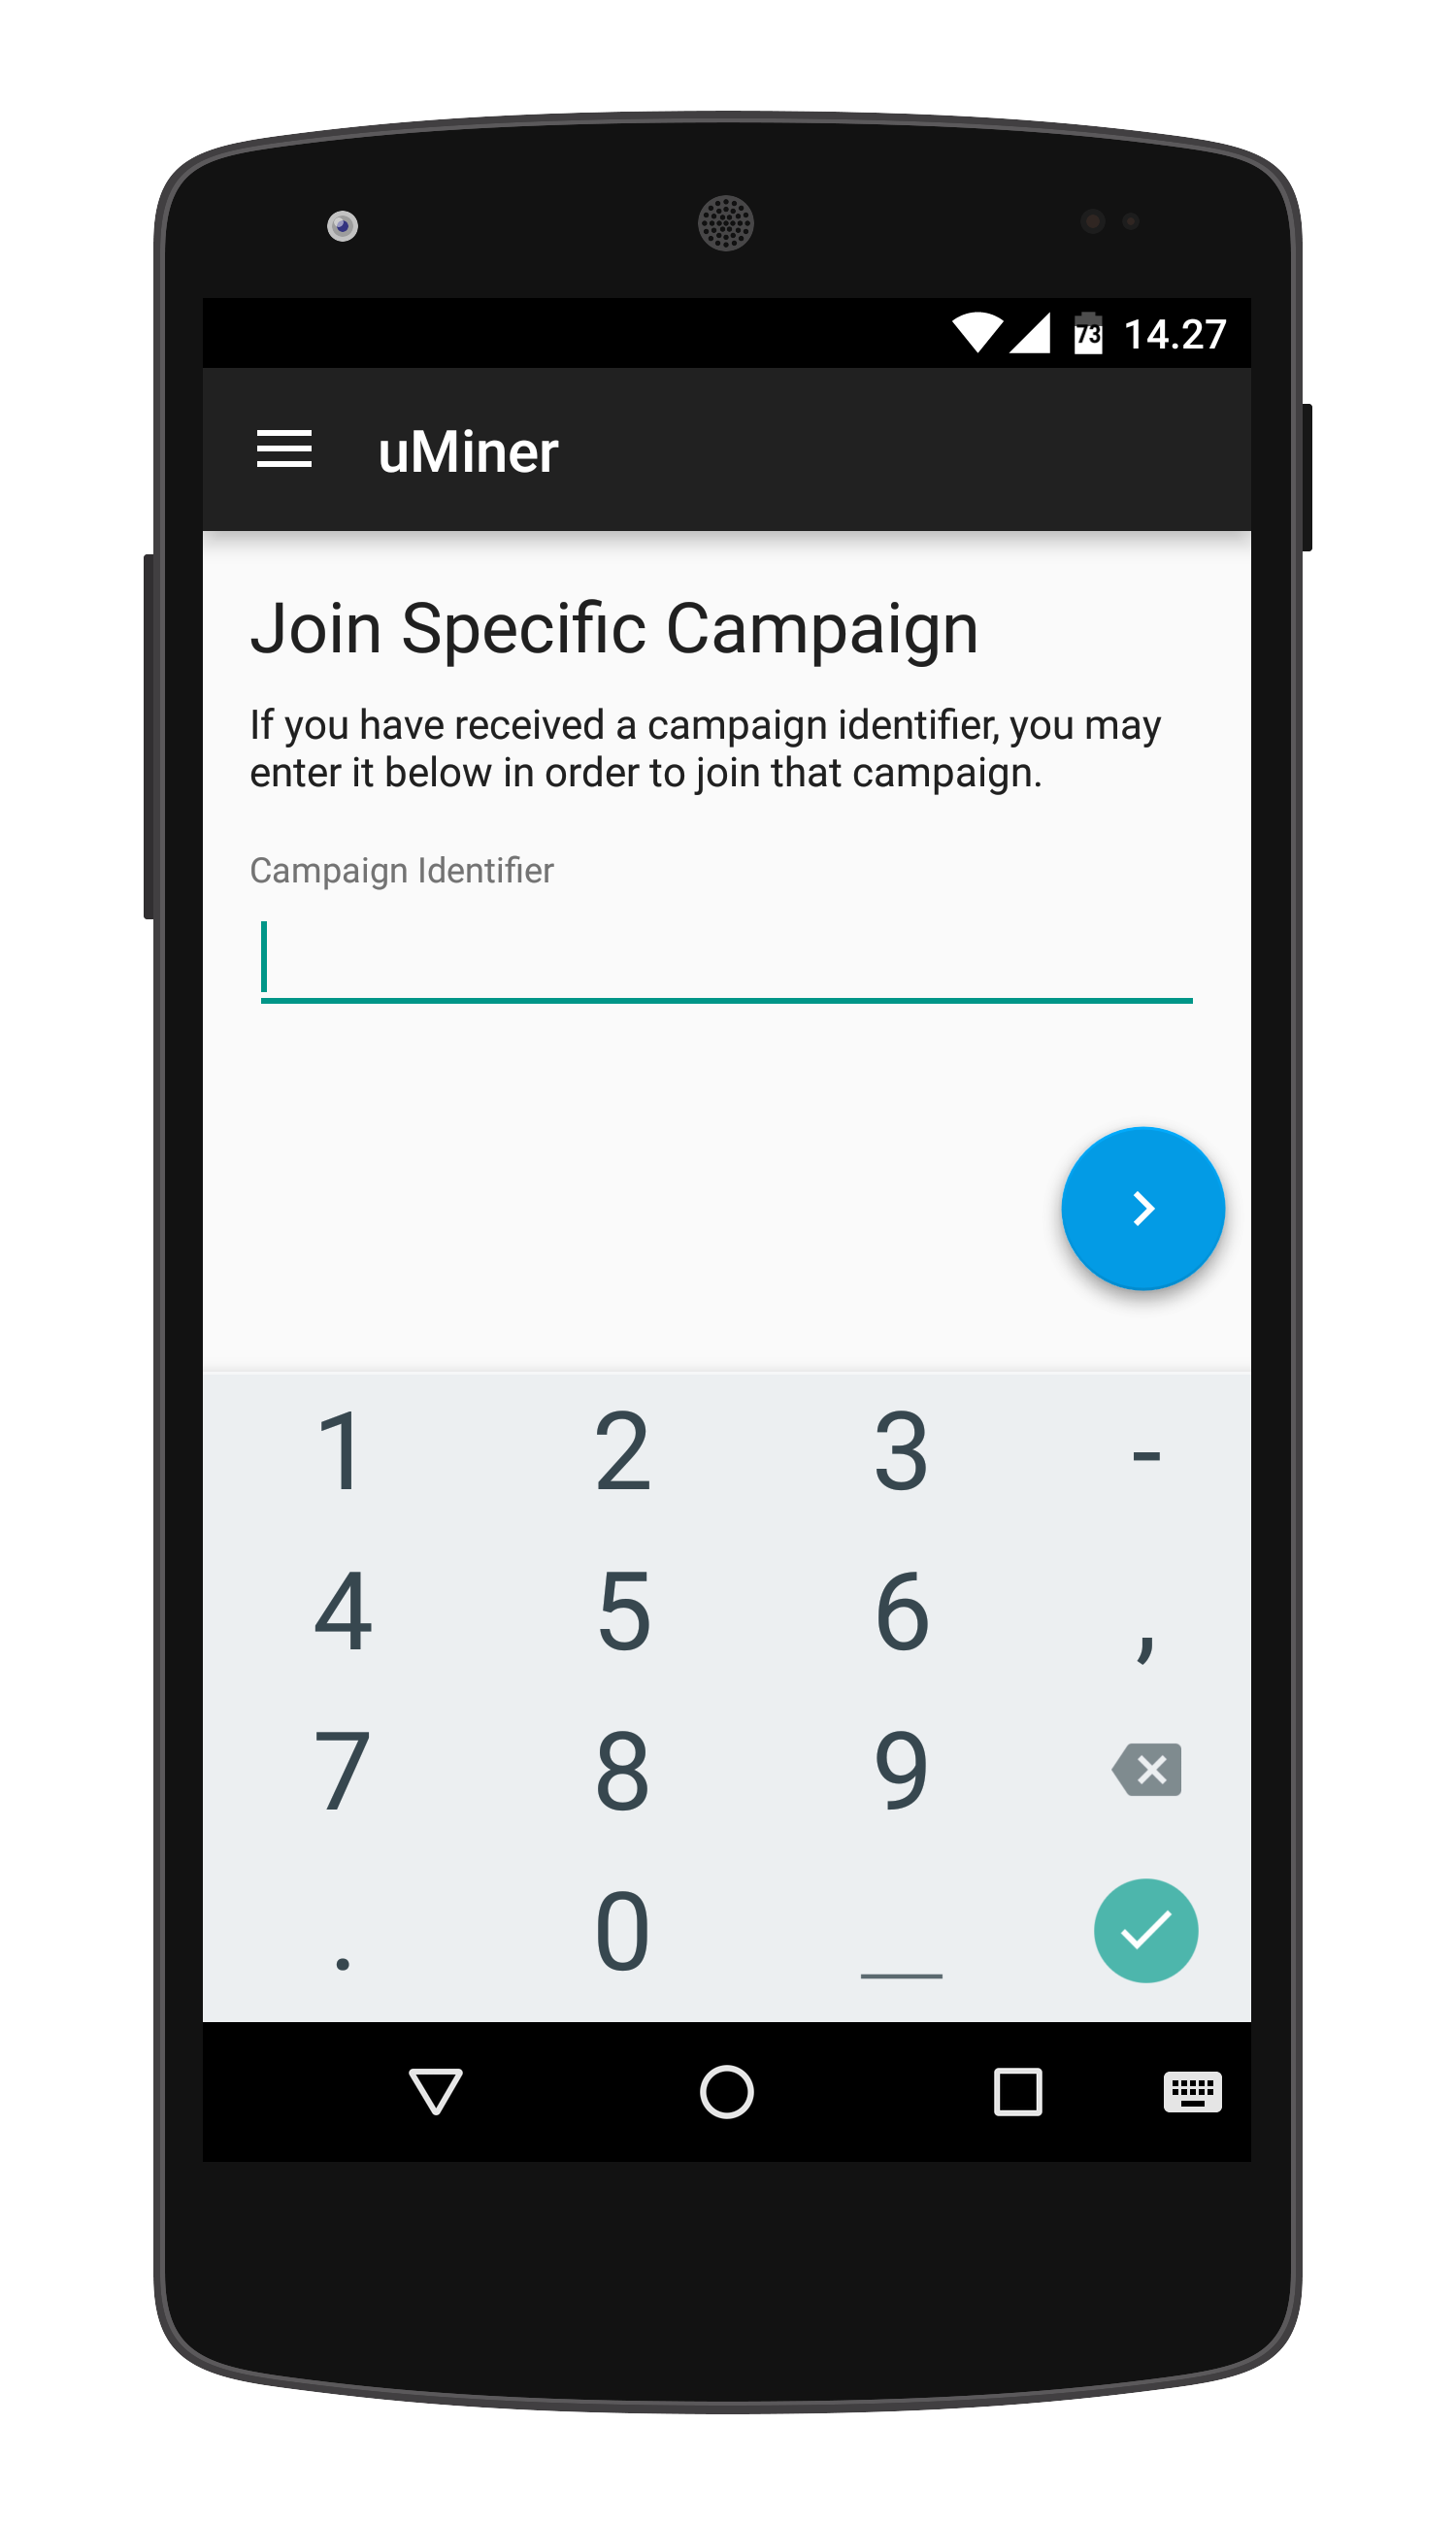
\includegraphics[width=.83\linewidth]{user_interfaces/client_join_specific_campaign_with_phone}
  \caption{Implementation.}
  \label{fig:implementation_specific_campaign}
\end{subfigure}
\caption{Search for a specific campaign using a campaign identifier.}
\label{fig:specific_campaign}
\end{figure}
\FloatBarrier

% Search for a campaign through a campaign identifier
\begin{figure}[!htbp]
\begin{subfigure}[!t]{.48\textwidth}
  \centering
  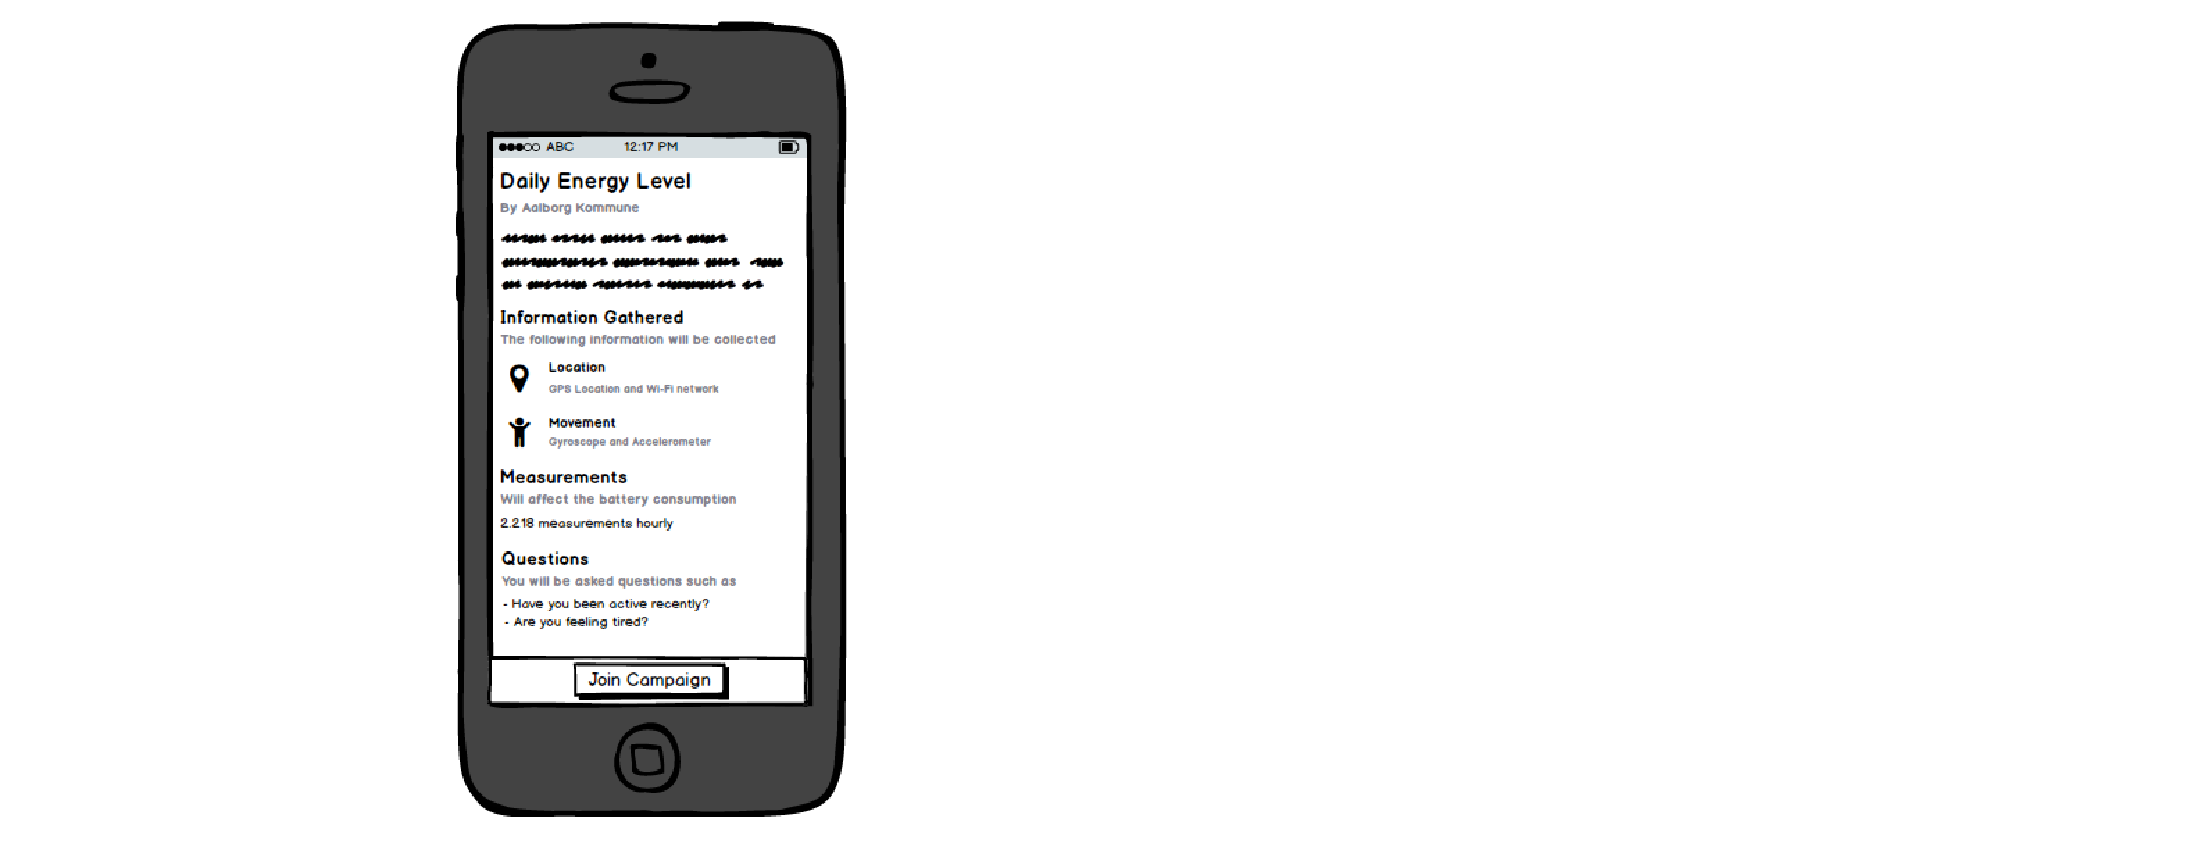
\includegraphics[width=.8\linewidth]{mockups/campaign_specification}
  \caption{Mockup.}
  \label{fig:mockup_campaign_specification}
\end{subfigure}%
\begin{subfigure}[!t]{.52\textwidth}
  \centering
  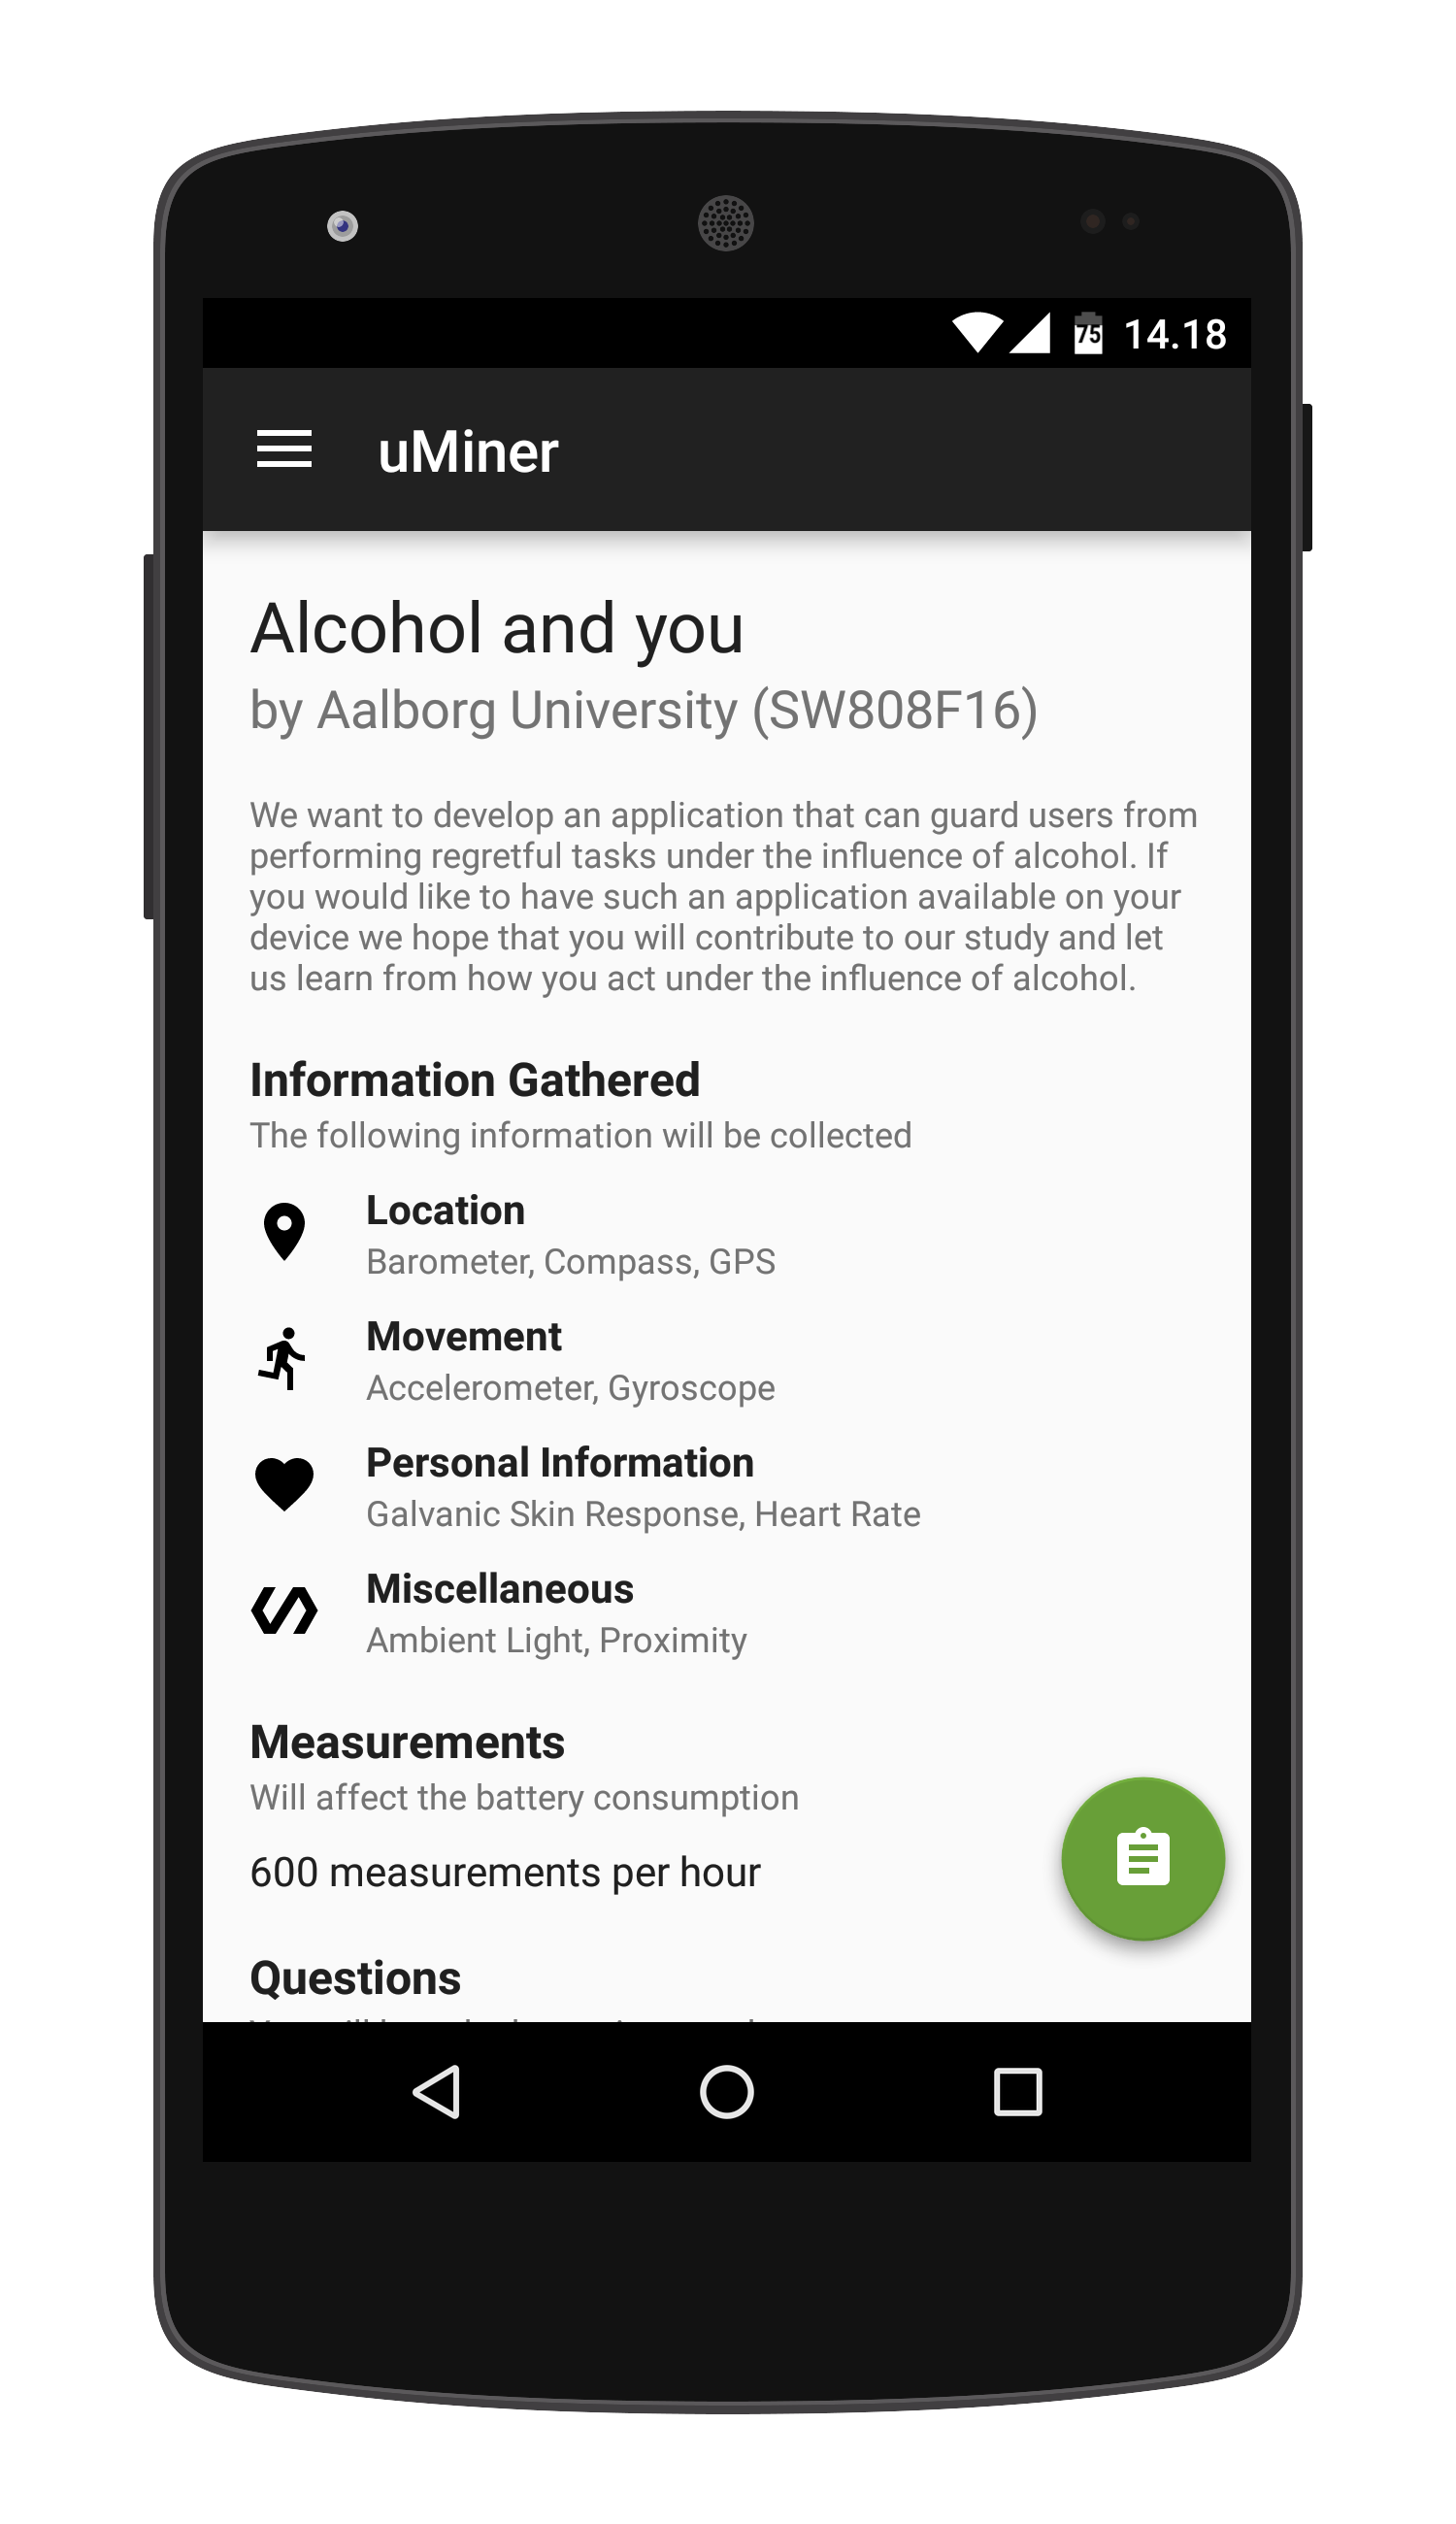
\includegraphics[width=.83\linewidth]{user_interfaces/client_campaign_specification2_with_phone}
  \caption{Implementation.}
  \label{fig:implementation_campaign_specification}
\end{subfigure}
\caption{Campaign specification view.}
\label{fig:campaign_specification}
\end{figure}
\FloatBarrier

% Answering questionnaires
\begin{figure}[!htbp]
\begin{subfigure}[!t]{.50\textwidth}
  \centering
  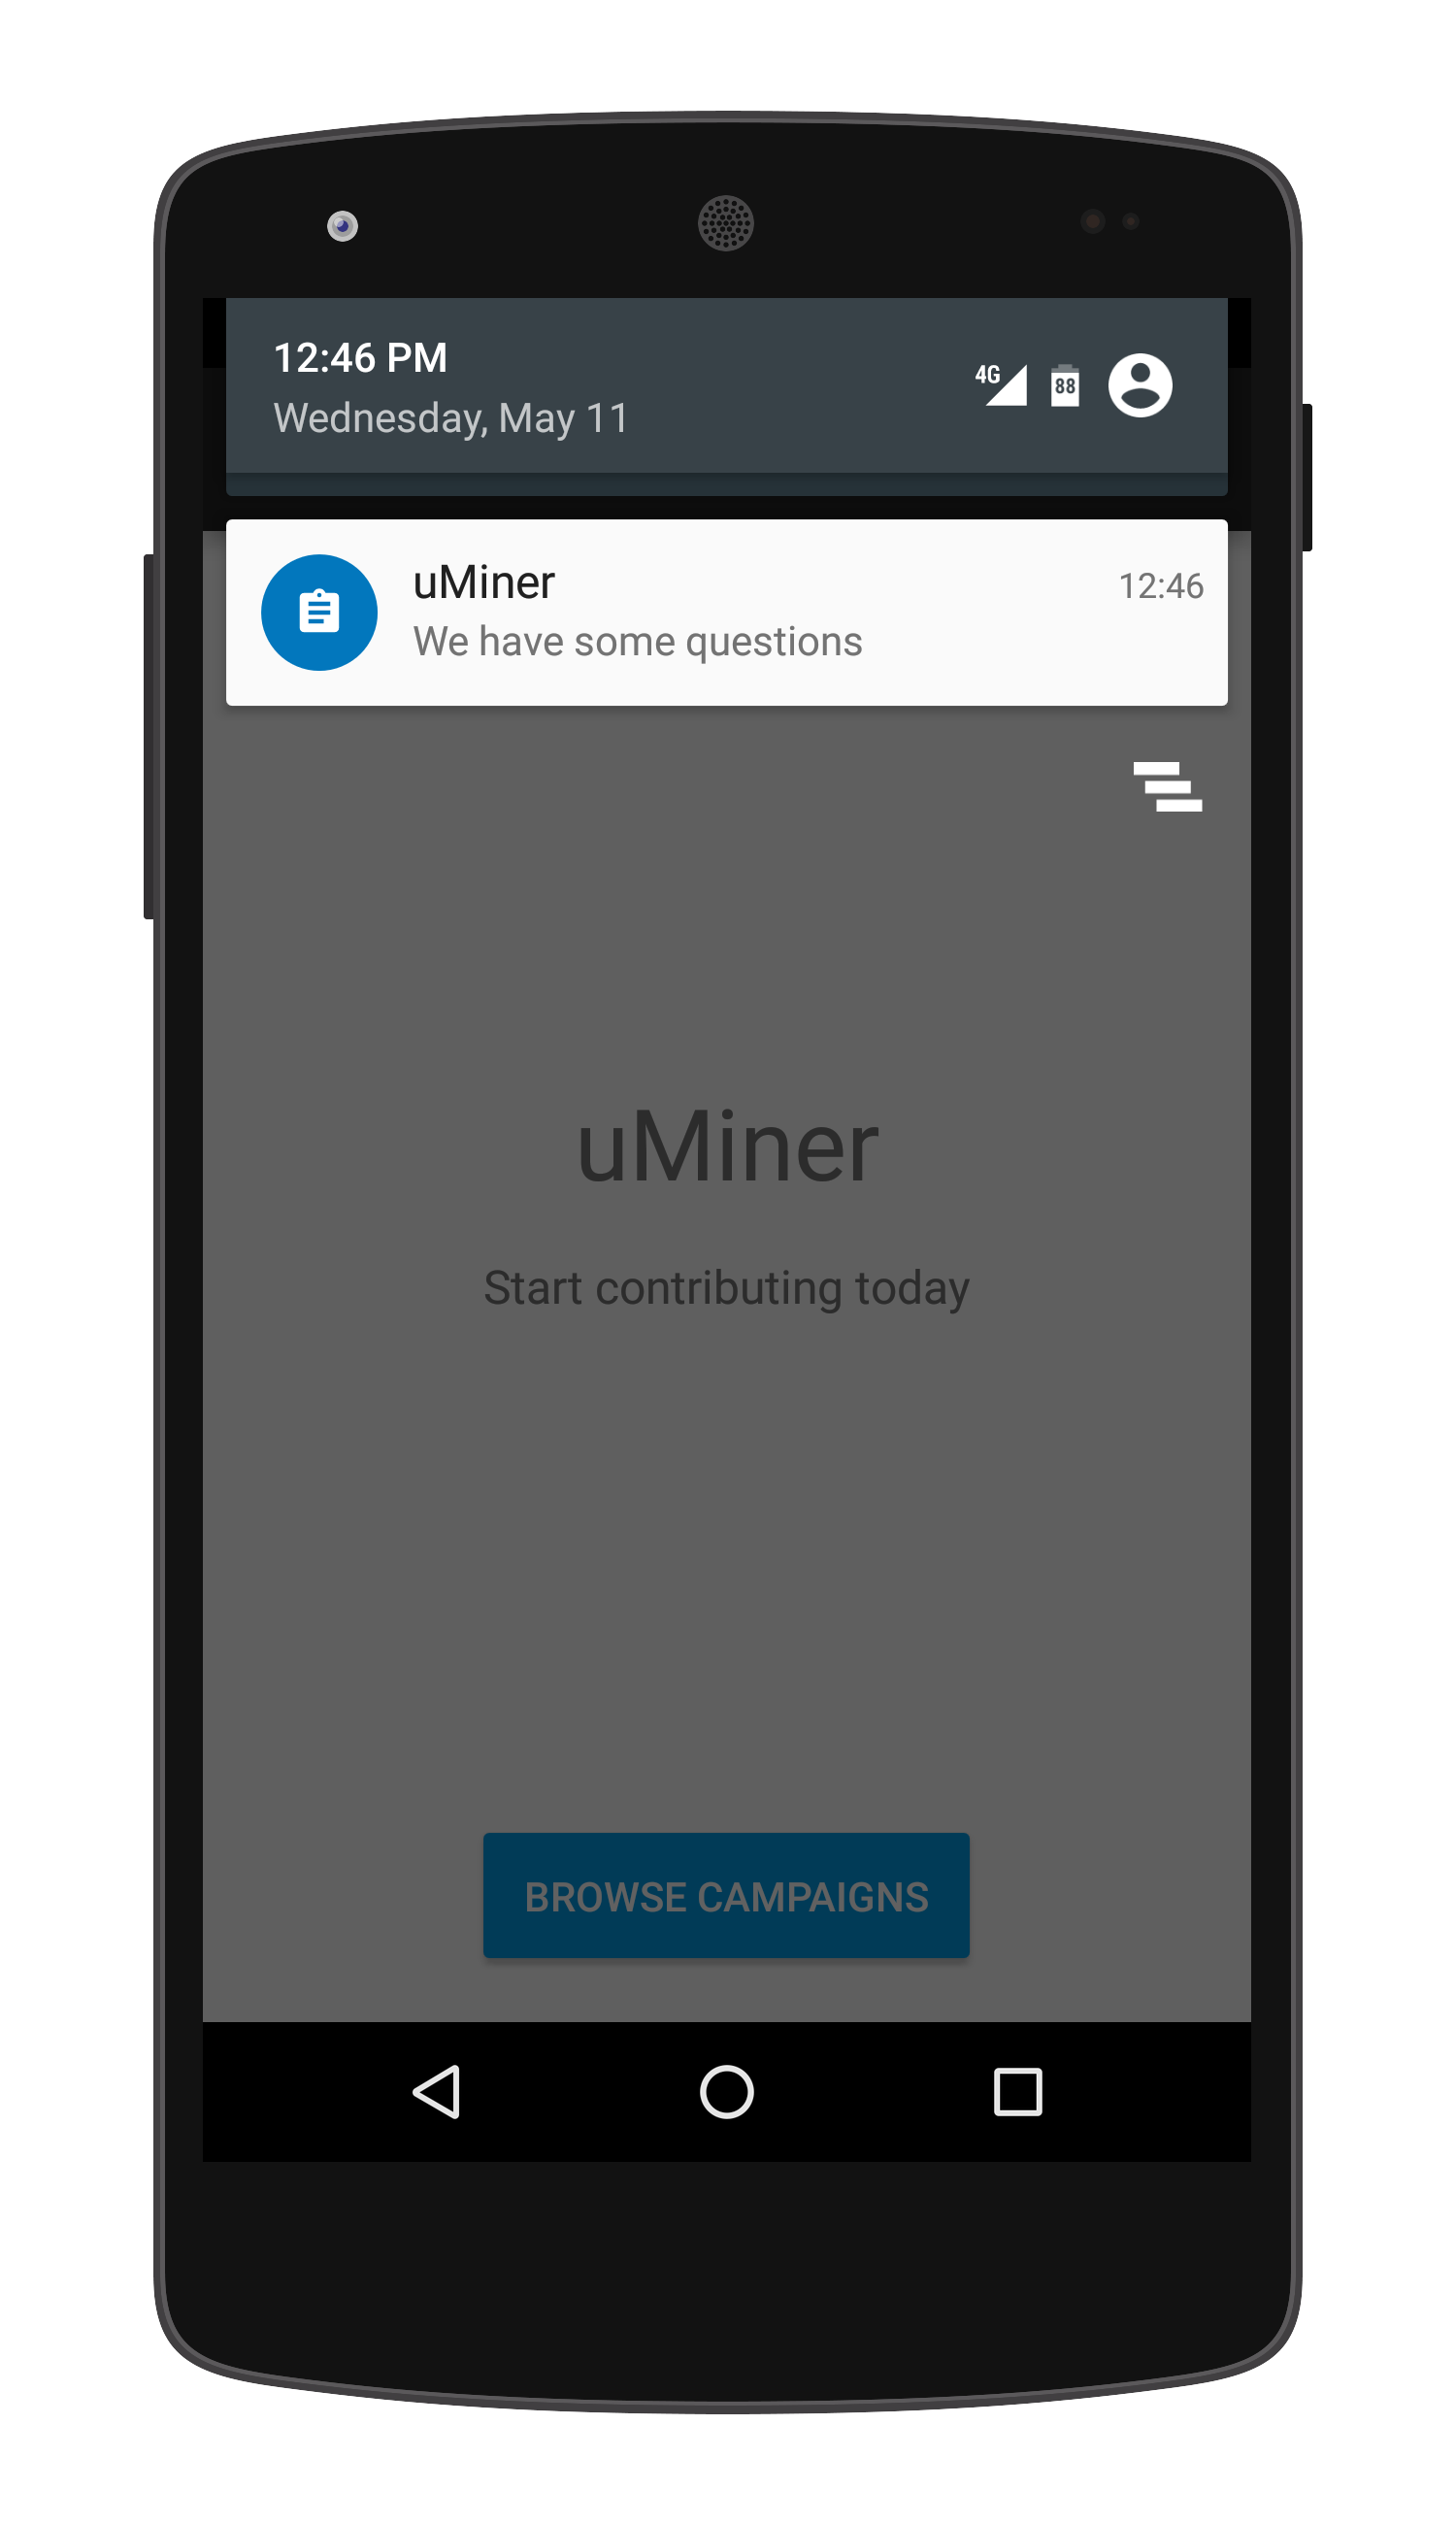
\includegraphics[width=.83\linewidth]{user_interfaces/client_notification_with_phone}
  \caption{Questionnaire notification.}
  \label{fig:answering_questionnaire_notification}
\end{subfigure}%
\begin{subfigure}[!t]{.50\textwidth}
  \centering
  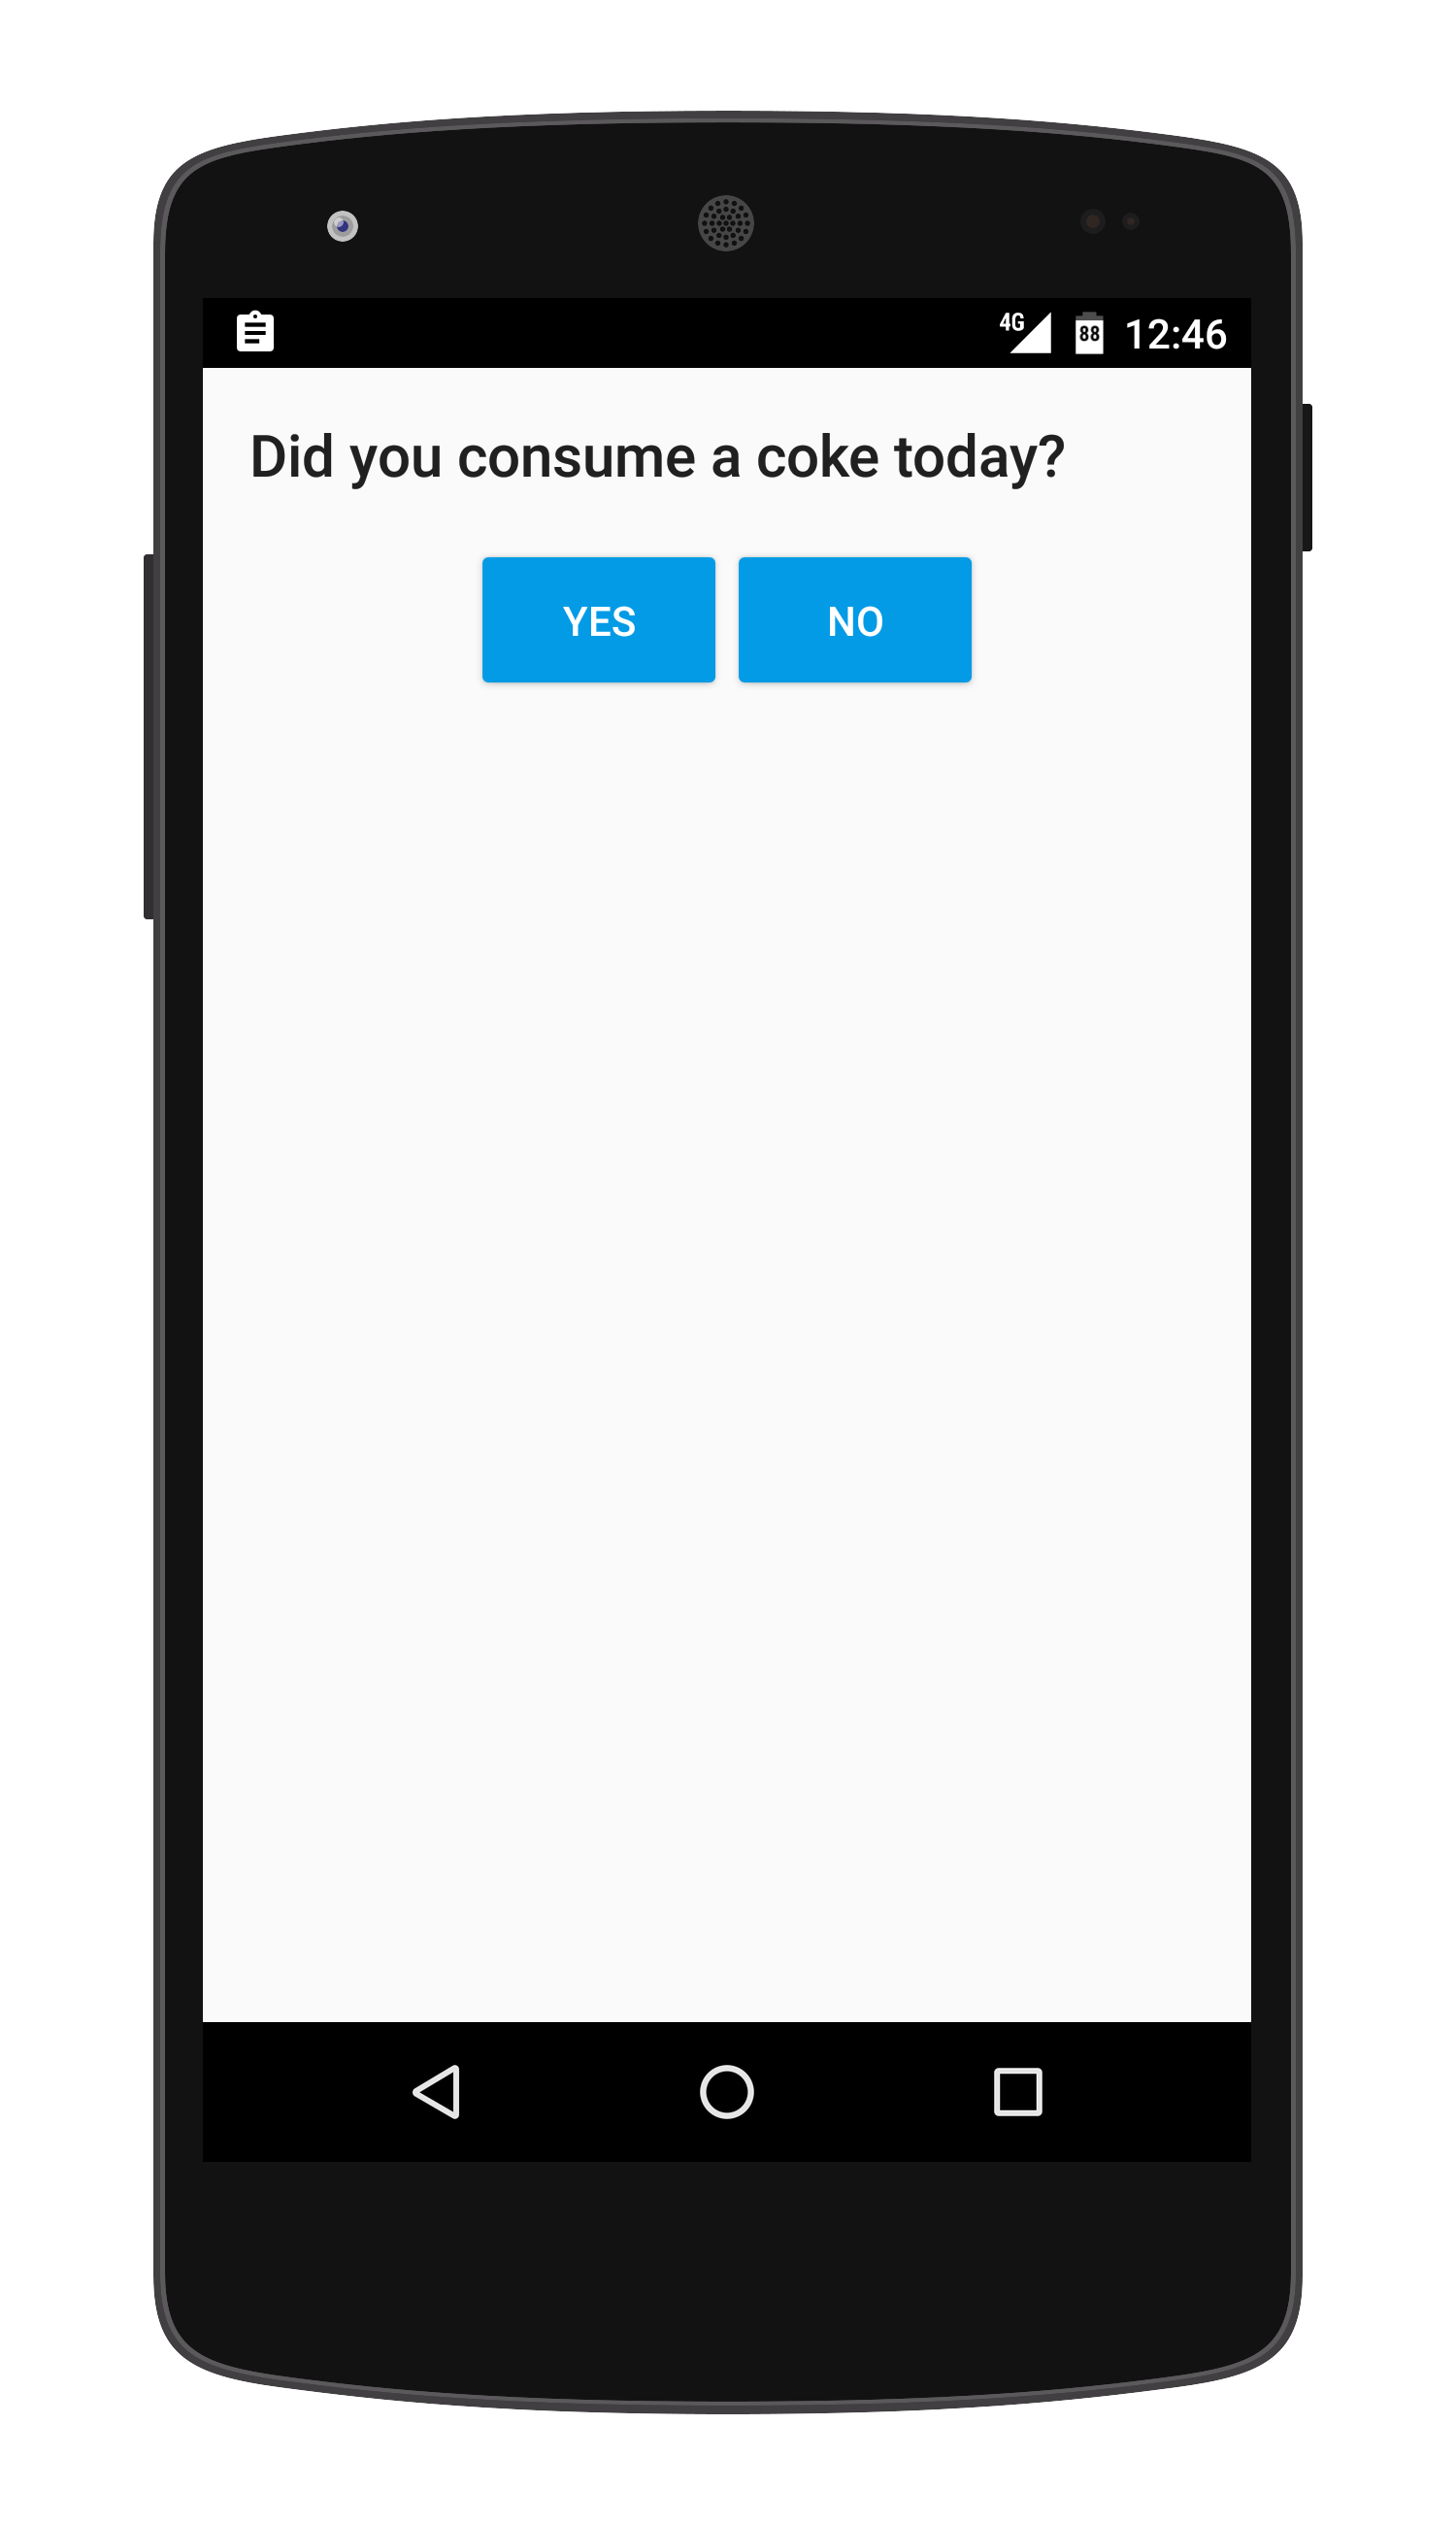
\includegraphics[width=.83\linewidth]{user_interfaces/client_answering_questions_with_phone}
  \caption{Answering the questionnaire.}
  \label{fig:answering_questionnaire_answering}
\end{subfigure}
\caption{Notification regarding questionnaire and answer view.}
\label{fig:answering_questionnaire}
\end{figure}
\FloatBarrier